% Beamer template
% Author: Ozgur Taylan TURAN
% Delft University of Technology

\documentclass[aspectratio=169]{beamer}
\usepackage{/Users/ozgurtaylanturan/Documents/TeXThemes/beamer/beamerthemetot}
% PACKAGES
\usepackage[english]{babel}
\usepackage{graphicx}
\usepackage{animate}
%\usepackage{calc}
\usepackage{calligra}
\usepackage[absolute,overlay]{textpos}
\usepackage[T1]{fontenc}
%\usefonttheme{serif}
\usefonttheme{professionalfonts}
\usepackage{amsmath}
\usepackage{palatino}
\usepackage{mathpazo}
\usepackage{graphicx}
%\usepackage{subfig}
\usepackage{tikz}
\usetikzlibrary{shapes,arrows}
\usepackage{xcolor}
\usepackage[T1]{fontenc}
%\usefonttheme{serif}
%\usepackage{titling}
\usepackage{graphicx}
%\usepackage{subfig}
%\usepackage{tikz}
%\usetikzlibrary{shapes,arrows}
\usepackage{mathtools}
\usepackage{cancel}
    
% BIB SETTINGS
\usepackage[backend=bibtex,firstinits=true,maxnames=30,maxcitenames=20,url=false,style=authoryear]{biblatex}
\bibliography{../../../Mendeley/bibtex/CoffeeTalks}

\setlength\bibitemsep{0.3cm} % space between entries in the reference list
\renewcommand{\bibfont}{\normalfont\scriptsize}
\renewcommand{\cite}[1]{\footnote<.->[frame]{\fullcite{#1}}}
\setbeamertemplate{bibliography item}{}

\setbeamertemplate{navigation symbols}{} % remove navigation symbols


 % COVER PAGE INFO   
\newcommand{\mytitle}{\color{White}\huge{\textbf{Coffee Talk \#2}}}
\newcommand{\mysubtitle}{\color{Pink}\Large{\textbf{The Deep Bootstrap Framework:Good Learners Are Good Offline Generalizers}}}
\newcommand{\myauthor}{\color{White}\textcalligra{\LARGE Ozgur Taylan Turan}}
\newcommand{\authorlabel}{\small O.T. Turan}
\author{\authorlabel}


\begin{document}
% COVER PAGE
{
{
\def\beamer@entrycode{\vspace*{-\headheight}}
\setbeamertemplate{frametitle}[default][center]
\setbeamertemplate{navigation symbols}{}
\usebackgroundtemplate{
\includegraphics[width=\paperwidth,height=\paperheight]{cover/coverart.pdf}}

\begin{frame}[plain] 

\begin{minipage}{\textwidth}
	\centering{\mytitle} \\
	%\vspace{1cm}
	%\centering{\mysubtitle} \\
	\vspace{1cm}
	\centering{\color{White}November 15, 2021} \\
	\vspace{1cm}
	\centering{\myauthor}\\
\end{minipage}
\end{frame}
}

\setbeamercovered{transparent}
\setbeamertemplate{footline}{\usebeamertemplate*{minimal footline}}
\setbeamertemplate{headline}{\usebeamertemplate*{minimal headline}}
\def\beamer@entrycode{\vspace*{-\headheight}}
}
% MAIN
\setbeamercovered{transparent}


\begin{frame}
	\centering
	\mysubtitle\cite{Nakkiran2020}
	Conference paper at 2021 ICLR
\end{frame}

\begin{frame}{Why This Paper?}
	\centering
	\begin{minipage}{0.5\textwidth}
			\centering
			 Interesting claims	
			 
			 \vspace{1cm}
			 Generalization $\leftrightarrow$ Optimization
	\end{minipage}
\end{frame}

\begin{frame}{Aim \& Problem Setting}
\begin{block}{\color{White} Aim}
	\begin{itemize}
		\item Create a framework for investigating generalization in interpolating regime TrainError $\approx$ 0
	\end{itemize}
		\centering
			TestError = $\cancelto{0}{\text{TrainError}}$ + ($\underbrace{\text{TestError}-\cancelto{0}{\text{TrainError}}}_{\text{Generalization gap}}$)
\end{block}
\begin{block}{\color{White} Problem Setting}
	\begin{itemize}
		\item Supervised classification:
 	\end{itemize}
 		\centering
 		$\mathcal{D}\sim(\mathbold{x},\mathbold{y})$ minimize training error with SGD variant on an architecture $\mathcal{F}$ for $t$ steps with the hope of a classifier $f_t$ with low testing error
\end{block}
\end{frame}

\begin{frame}{Real World vs Ideal World-A}

For a fixed $\mathcal{D}$ and $\mathcal{F}$:

\centering 
\begin{minipage}{0.4\textwidth}
	\begin{block}{\color{White}Ideal World [Train$_{\mathcal{D,F}}(\infty ,t)$]}
		\begin{itemize}
			\item Access to $\mathcal{D}$
			\item Take $t$ steps on mini-batches sampled from $\mathcal{D}$ to get $f_t^\text{iid}$
		\end{itemize}
	\end{block}	
\end{minipage}%
\hspace{1cm}
\begin{minipage}{0.4\textwidth}
		\begin{block}{\color{White}Real World [Train$_{\mathcal{D,F}}(n,t)$]}
		\begin{itemize}
			\item Access to $n$ samples from $\mathcal{D}$
			\item Take $t$ steps on mini-batches of $n$ samples to get $f_t$
		\end{itemize}
	\end{block}
\end{minipage}

\vspace{1cm}
\centering
	TestError($f_t$) = TestError($f_t^{\text{iid}}$) + $\underbrace{\text{(TestError($f_t$) - TestError($f_t^{\text{iid}}$))}}_{\text{Bootstrap error} (\varepsilon)}$
\end{frame}

\begin{frame}{Real vs Ideal-B}
	\begin{itemize}
		\item So keeping everything same,
	\end{itemize}
		\centering
		\textbf{Ideal World} $\to$ minimize population loss
		
		\textbf{Real World} $\to$ minimize empirical loss
		
		\vspace{1cm}
		\color{Pink} Claim: \color{Black} $\varepsilon(n,\mathcal{D,F},t)$ is small for all \textit{realistic} ($n,\mathcal{D,F}$) at all $t$
\end{frame}

\begin{frame}{Experimental Setup}
\begin{block}{\color{White} Datasets}
	\begin{itemize}
		\item CIFAR-5m: generating 6M synthetic data 5M:train 1M:test
	\end{itemize}	
\end{block}
\begin{block}{\color{White} Training}
	\begin{itemize}
		\item Train the real world optimizer until $\leq1\%$ or reach specified epochs
	\end{itemize}	
\end{block}
\begin{block}{\color{White} Measure}
	\begin{itemize}
		\item Soft-Error = 1 - softmax(correct label)
	\end{itemize}	
\end{block}

\centering
\color{Pink} If we have 10 points for training and train for 2 epochs in Real world then, I have to get 20 unique samples and train for 1 epoch for the Ideal world
\end{frame}

\begin{frame}{Results-A}
	\centering
	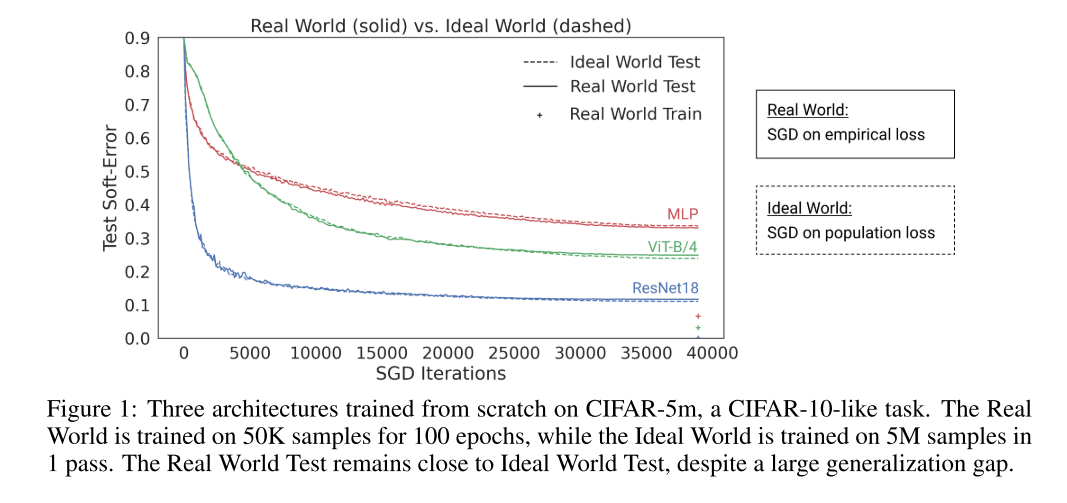
\includegraphics[width=0.8\textwidth]{Figures/1}
		
	\color{Pink} Claim: \color{Black} Generalization gap MLP $\geq$ CNN because CNN optimize faster in the Ideal world.
\end{frame}

\begin{frame}{Results-B}
	\centering
	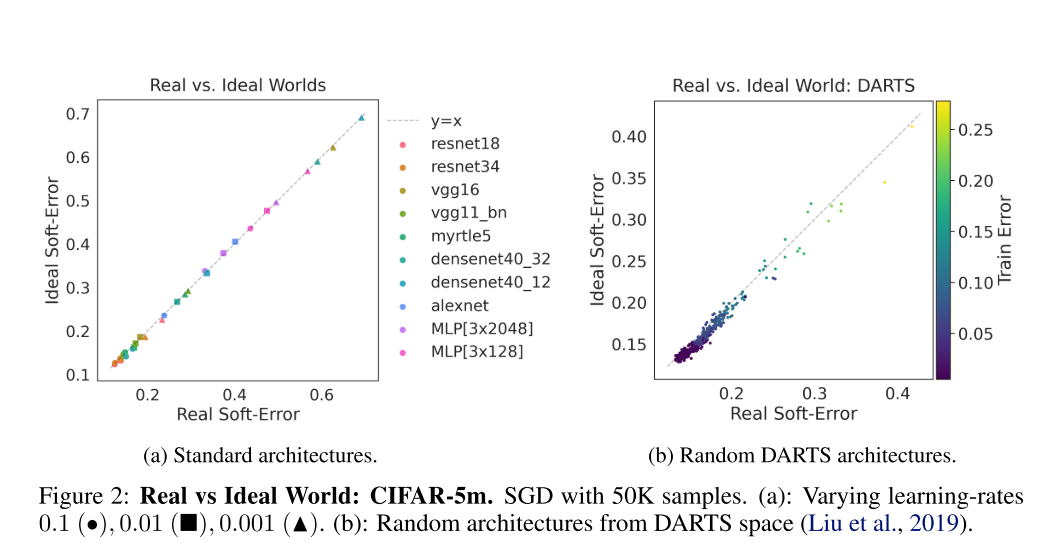
\includegraphics[width=0.8\textwidth]{Figures/2}	
\end{frame}

\begin{frame}{Results-C}
	\centering
	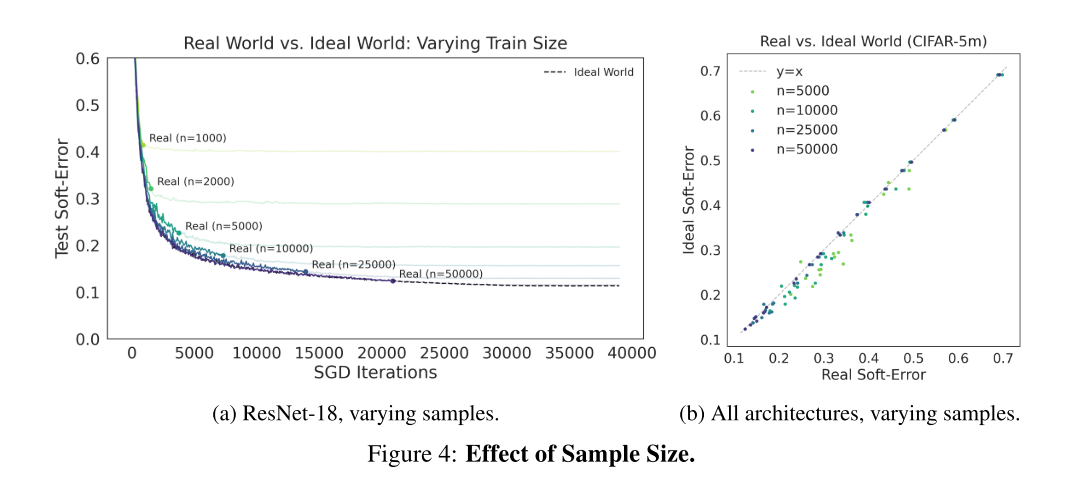
\includegraphics[width=0.8\textwidth]{Figures/4}
\end{frame}

\begin{frame}{Conclusions}
\begin{itemize}
	\item To understand the generalization (offline performance) in DL one has to look to population loss (online learning) has to be investigated
	\item Test performance of modern settings is close between infinite and finite sample sizes $\to$ quick online learners are well generalizers ?
\end{itemize}	
\end{frame}


\end{document}